\documentclass{article}
% --- Modify margins --- %
\usepackage{geometry}
\geometry{a4paper,scale=0.8}
% --- Involved packages --- %
\usepackage{amssymb}
\usepackage{enumitem}
\usepackage{amsthm}
\usepackage{amsmath}
\usepackage{bm}
\usepackage{graphicx}
\usepackage{physics}
\usepackage{enumitem}
\usepackage{listings}
\usepackage{xcolor}
\usepackage[utf8]{inputenc}
\usepackage[english]{babel}
\usepackage{appendix}

\renewcommand{\familydefault}{\sfdefault}

\definecolor{codegreen}{rgb}{0,0.6,0}
\definecolor{codegray}{rgb}{0.5,0.5,0.5}
\definecolor{codepurple}{rgb}{0.58,0,0.82}
\definecolor{backcolour}{rgb}{0.95,0.95,0.92}

\lstdefinestyle{mystyle}{
    % backgroundcolor=\color{backcolour},   
    commentstyle=\color{codegreen},
    keywordstyle=\color{magenta},
    numberstyle=\tiny\color{codegray},
    stringstyle=\color{codepurple},
    basicstyle=\sffamily\footnotesize,
    breakatwhitespace=false,         
    breaklines=true,                 
    captionpos=b,                    
    keepspaces=true,                 
    % numbers=left,                    
    numbersep=5pt,                  
    showspaces=false,                
    showstringspaces=false,
    showtabs=false,                  
    tabsize=2
}

\lstset{style=mystyle}

% --- NewCommand --- %
% \newcommand{\norm}[1]{\left\lVert#1\right\rVert}

\usepackage{hyperref}
\hypersetup{
    colorlinks=true,
    linkcolor=blue,
    filecolor=magenta,      
    urlcolor=cyan,
}

\urlstyle{same}




% --- Title information --- %
\title{CS 760: Machine Learning - Fall 2020\\
        {\Large \textbf{Homework 5: Nearest Neighbors \& Naive Bayes}}\\
        {\normalsize \textbf{Due : 11/12/2020}}
    }
\author{Zijie Zhang}
\date{\today}


% --- main --- %

\begin{document}
    \maketitle
    % Problem 1
    \section*{Problem 1}
    \begin{enumerate}[label=(\alph*)]
        \item I chose the KNN variant that,\\
            weights = 'uniform', metric = 'euclidean'\\
            The data should be min-max normalized before computing.
            The Accuracy is 81\%.\\
            \textbf{KNN.py} = \url{https://github.com/z-zijie/2020Fall/tree/master/COMP760/Homework5}
        \item Euclidean distance. Because this metric is more intuitive.
        \item \indent
        \begin{center}
            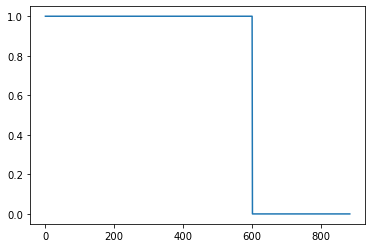
\includegraphics[width=9cm]{1c.png}
        \end{center}
        \item The best choice of K is 5.
        \item We can use the voting ratio to decide reliability.
    \end{enumerate}
    

    % Problem 2
    \section*{Problem 2}
    \begin{enumerate}[label=(\alph*)]
        \item \textbf{Bayes.py} = \url{https://github.com/z-zijie/2020Fall/tree/master/COMP760/Homework5}
        \item Passenger Class, Gender, Siblings/Spouses and Parents/Children are Bernoulli.\\
        Age and Fare are Gaussian.
        \item x = [1, 1, 22, 1, 0, 71.2833], survived.
        \item If prediction=survived, confidence = $P(\text{survived}|x)/P(\text{survived}|x) + P(\text{NOT survived}|x)$.
    \end{enumerate}


    % Problem 3
    \section*{Problem 3}
        I prefer Random Forest, because this algorithm is very interpretable.
\pagebreak
\appendix
\section*{KNN}
\lstinputlisting[language=Python]{KNN.py}
\section*{Bayes}
\lstinputlisting[language=Python]{Bayes.py}
\end{document}